\documentclass[ENG, BIB]{TFUOC}%IB: CASTELLANO, CAT: CATALÁN, ENG: ANGLÈS

%%%%%%%%%%%%%%%%%%%%%%%%%%%%%%%%%%%%%%%%%%%%%%%%%%%%%%%%%%%%%%%%%%%%%%
%%---------------------------- PACKAGES ----------------------------%%
%%%%%%%%%%%%%%%%%%%%%%%%%%%%%%%%%%%%%%%%%%%%%%%%%%%%%%%%%%%%%%%%%%%%%%

\usepackage{titlesec}
\titleformat{\chapter}[hang]
  {\bfseries\color{darkblueUOC} \Huge}
  {\thechapter.}
  {1em}
  {}

\titlespacing{\chapter}{0pt}{-10pt}{50pt}
\usepackage{mathpazo} % Use the Palatino font by default
\usepackage[autostyle=true]{csquotes} % Required to generate language-dependent quotes in the bibliography
\usepackage{hyperref}
\usepackage{bookmark}
\usepackage{booktabs}
\usepackage[table,xcdraw]{xcolor}
\usepackage{pgfgantt}
\hypersetup{
    colorlinks=true,
    linkcolor=blue,
    filecolor=magenta,      
    urlcolor=cyan,
    pdftitle={Memoria},
    pdfpagemode=FullScreen,
    }
\usepackage[backend=biber, style=nature]{biblatex}
\addbibresource{library.bib}
\addbibresource{packages.bib}
% \bibliography{library.bib}
\urlstyle{same}
\usepackage[toc, acronym, xindy]{glossaries}
\makeglossaries
\loadglsentries[main]{glossary.tex}

\usepackage{lscape}
    
    %%%%%%%%%%%%%%%%%%%%%%%%%%%%%%%%%%%%%%%%%%%%%%%%%%%%%%%%%%%%%%%%%%%%%%
    %%-------------- TEMP DOCUMENT SETTINGS FOR COMMENTS ---------------%%
    %%%%%%%%%%%%%%%%%%%%%%%%%%%%%%%%%%%%%%%%%%%%%%%%%%%%%%%%%%%%%%%%%%%%%%
\usepackage[colorinlistoftodos, textwidth=65mm, shadow]{todonotes}


    
    %%%%%%%%%%%%%%%%%%%%%%%%%%%%%%%%%%%%%%%%%%%%%%%%%%%%%%%%%%%%%%%%%%%%%%
    %%---------------------------- PREAMBLE ----------------------------%%
    %%%%%%%%%%%%%%%%%%%%%%%%%%%%%%%%%%%%%%%%%%%%%%%%%%%%%%%%%%%%%%%%%%%%%%
    
    %Introducción de datos del trabajo
    \title{metaboPipe: a Modular Pipeline for Metabolomic Data Preprocessing}
    \titcrt{metaboPipe} %Título corto que aparecerá a la cabecera
    \author{Eduard Pérez Méndez}
    \date{\today}
    
    
    \nomPDC{Alexandre Sánchez Pla}
    \nomPRA{Carles Ventura Royo}
    \titulac{Master's degree in Bioinformatics \newline and Biostatistics}
    \area{Statistical Bioinformatics and \newline Machine Learning}
    \idioma{English}
    \credits{15}
    \parcla{targeted metabolomics, preprocessing, pipeline}
    
    \licenc{ccByNcSa}
    %Posibles licencias
    %ccByNcNd
    %ccByNcSa
    %ccByNc
    %ccByNd
    %ccBySa
    %ccBy
    %GNU
    %copyright
    
    
    %%%%%%%%%%%%%%%%%%%%%%%%%%%%%%%%%%%%%%%%%%%%%%%%%%%%%%%%%%%%%%%%%%%%%%
    %%---------------------------- ABSTRACT ----------------------------%%
    %%%%%%%%%%%%%%%%%%%%%%%%%%%%%%%%%%%%%%%%%%%%%%%%%%%%%%%%%%%%%%%%%%%%%%
    
    % \abstractidioma{
        % Máximo 250 palabras, con la finalidad, contexto de aplicación, metodología, resultados y conclusiones del trabajo.
        % }
        
        % Resumen en inglés.
        \abstractenglish{
            A maximum of 250 words, detailing the purpose, contexto of application, methodology, results and conclusiones of the work.
            }
            
            
            %%%%%%%%%%%%%%%%%%%%%%%%%%%%%%%%%%%%%%%%%%%%%%%%%%%%%%%%%%%%%%%%%%%%%%
            %%---------------------------- BEGINDOC ----------------------------%%
            %%%%%%%%%%%%%%%%%%%%%%%%%%%%%%%%%%%%%%%%%%%%%%%%%%%%%%%%%%%%%%%%%%%%%%
            \begin{document}
            
            \estructura
            
            %%%%%%%%%%%%%%%%
            %--- THANKS ---%
            %%%%%%%%%%%%%%%%
            \newpage\null\thispagestyle{empty}
            
            \vspace*{0.4\textheight} 
            
            \noindent\enquote{\itshape BIG MOTIVATIONAL QUOTE
            }\bigbreak 
            
            % People think of education as something they can finish - Isaac Asimov
            
            % Self-education is, I firmly believe, the only kind of education there is. - Isaac Asimov
            
            % Never let your sense of morality stop you from doing the right thing. - Isaac Asimov

            \hfill AUTHOR NAME
            
            \newpage
            
            
            % --- TABLE OF CONTENTS --- %
            \tableofcontents
            
            % --- LIST OF FIGURES --- %
\listoffigures

% --- LIST OF TABLES --- %
\listoftables



%%%%%%%%%%%%%%%%%%%%%%%%%%%%%%%%%%%%%%%%%%%%%%%%%%%%%%%%%%%%%%%%%%%%%%%%%%
%%---------------------------- INTRODUCTION ----------------------------%%
%%%%%%%%%%%%%%%%%%%%%%%%%%%%%%%%%%%%%%%%%%%%%%%%%%%%%%%%%%%%%%%%%%%%%%%%%%
\chapter{Introduction}

\section{General description}

Metabolomics, a powerful and evolving field within the realm of systems biology, plays a pivotal role in unraveling the intricate web of biochemical processes occurring within living organisms. As we delve into the molecular intricacies of biological systems, the generation of vast and complex datasets poses a significant challenge. Challenges in standardizing nutritional metabolomics include experimental design, sample preparation, and data analysis, which impact result validity and reproducibility. Efforts by the international community aim to establish standard procedures and infrastructure for advancing nutritional metabolomics research. This master thesis project aims for the creation of a modular pipeline designed to streamline the processing of targeted metabolomics data to a usable and meaningful dataset for further analysis and biological interpretation.

\section{Context and justification}

Metabolomics is a rapidly evolving field within biology that focuses on the comprehensive study of the metabolite composition of cell types, tissues, organs, or organisms \cite{pattiMetabolomicsApogeeOmics2012,zhangSerumMetabolomicsNovel2012,chenGuideMetabolomicsAnalysis2022a}. It aims to measure, identify and (semi-)quantify those metabolites. Metabolites are chemical compounds that undergo analysis through conventional chemical assessment methods like \acrfull{ms} and \acrfull{nmr} spectrometry. \acrshort{ms} approaches are commonly integrated with \acrfull{gc} and \acrfull{lc}, leading to the development of two advanced techniques known as \acrfull{gcms} and \acrfull{lcms}. All of these analytical platforms and methodologies generate large amounts of high-dimensional and complex experimental raw data.

However, the statistical analysis of metabolomics data presents significant challenges, attributable not only to the inherent complexity of metabolomics as a research discipline but also to the intricate nature of the data itself. Notwithstanding that numerous studies have explored various methodologies for metabolomic data management, the field still lacks an accepted standard for preprocessing and pretreatment of such data.

One of the obstacles the field encounters is the lack of well defined terminology, as the terms “data preprocessing” and “data pretreatment” have not been used consistently in metabolomics literature \cite{sunPretreatingNormalizingMetabolomics2024}.

The objectives of data preprocessing/pretreatment encompass two primary aims: firstly, to rectify or mitigate instrumental artifacts and extraneous biological variance, thereby amplifying the \acrfull{snr}; and secondly, to effectively transform the data into interpretable spectral profiles through processes such as centering, scaling, and dimensionality reduction \cite{sunPretreatingNormalizingMetabolomics2024,martinPepsNMR1HNMR2018}. The choice of preprocessing and pretreatment methods can significantly impact the downstream analysis and interpretation of metabolomic data \cite{karamanPreprocessingPretreatmentMetabolomics2017} so the steps should be carefully selected based on the specific characteristics of the data and the research.

By establishing a standardized approach to preprocess and pretreat metabolomic data, the field can improve the quality, comparability, and reproducibility of metabolomic studies. This would facilitate data integration, enable the development of robust statistical models, and enhance our understanding of the complex metabolic processes underlying health and disease.


\subsection{Preprocessing of data}

Given the inherent dissimilarities in data acquisition techniques, unique preprocessing procedures are imperative before embarking on statistical analyses in metabolomics investigations. \acrshort{nmr} spectra, for instance, often exhibit signal shifts along the axis due to factors like pH fluctuations \cite{bhinderwalaChemicalShiftVariations2022}. Thus, meticulous preprocessing is indispensable to ensure robust statistical analyses and facilitate inter-spectral signal comparisons. This involves techniques such as binning, peak fitting with spectral databases, and exclusion of unstable or non-informative spectral regions (e.g., water peaks) \cite{chenGuideMetabolomicsAnalysis2022a,sunPretreatingNormalizingMetabolomics2024,stanstrupMetaRbolomicsToolboxBioconductor2019}. By refining the dataset to a subset of relevant metabolites, statistical methods can effectively discern variations in signal intensity among sample groups \cite{qiuSmallMoleculeMetabolites2023}.


The preprocessing workflows diverge between \acrshort{ms}-based and \acrshort{nmr}-based metabolomic analyses. In \acrshort{ms}-based profiling, data are presented as three-dimensional (3D) tables, in contrast to the two-dimensional (2D) tables derived from GC-MS data preprocessing \cite{sunPretreatingNormalizingMetabolomics2024,stanstrupMetaRbolomicsToolboxBioconductor2019}. \acrshort{gcms} preprocessing entails deconvolution and peak integration to generate intensity profiles for each sample feature corresponding to {RT/m/z} pairs. Notably, metabolite identification strategies differ between \acrshort{gcms} and \acrshort{lcms} methodologies. While \acrshort{gcms} relies on reproducible mass spectra and extensive databases for metabolite identification based on characteristic fragment ions, \acrshort{ms}-based methods prioritize automation, accuracy, peak identification, integration, and annotation \cite{xiaoMetaboliteIdentificationQuantitation2012,kiselevaDefiningBloodPlasma2021}.


While the primary objective of preprocessing is to render data comparable across samples despite instrumental discrepancies, the strategies employed in \acrshort{ms}-based methodologies differ from those in \acrshort{nmr}-based approaches. Moreover, variations exist between preprocessing methodologies utilized in \acrshort{gcms} and \acrshort{lcms} metabolomic analyses, underscoring the intricate nature of metabolomics data preprocessing.


\subsubsection{MS-based data preprocessing}

\acrshort{ms}-based analysis involves the measurement of \acrfull{mz}. When combined with either \acrshort{lc} or \acrshort{gc}, the resulting raw GC/LC-MS data encompass three measured variables: \acrshort{mz}, chromatographic \acrfull{rt}, and intensity count, thereby constituting a three-dimensional (3D) data structure.
To streamline the data and eliminate spectral noise and irrelevant biological variability, a two-dimensional (2D) features table is generated through peak picking. This table encompasses all quantified metabolic features from the analyzed samples, with rows corresponding to samples and columns representing variables such as peak areas or intensities, characterized by m/z and retention time in minutes or scan number (m/z-RT pairs).
The preprocessing of \acrshort{ms} data involves several steps: 1) denoising and baseline correction; 2) alignment across all samples; 3) peak picking; 4) merging the peaks; and 5) creating a data matrix \cite{chenGuideMetabolomicsAnalysis2022a,sunPretreatingNormalizingMetabolomics2024,xiaoMetaboliteIdentificationQuantitation2012, defernezChapterElevenStrategies2013,troisiChapterDataAnalysis2022,burtonInstrumentalExperimentalEffects2008,trygg01BackgroundEstimation2009,alonsoAnalyticalMethodsUntargeted2015,bloembergWarpingMethodsSpectroscopic2013}.


\subsubsection{NMR-based data preprocessing}
Similar to \acrshort{ms}-based analysis, \acrshort{nmr}-based analysis generates a 2D structure of feature data matrix with the samples in the rows and the spectral data points in the columns. Also similar to \acrshort{ms}-based analysis, the \acrshort{nmr}-based analysis (e.g., 1H NMR analysis) requires data preprocessing to mitigate non-biologically relevant effects. The following data preprocessing steps could be performed: 1) baseline correction; 2) peak binning; 3) peak alignment; 4) quality control; 5) create a data matrix \cite{sunPretreatingNormalizingMetabolomics2024,martinPepsNMR1HNMR2018,trygg01BackgroundEstimation2009,alonsoAnalyticalMethodsUntargeted2015,bloembergWarpingMethodsSpectroscopic2013,borkChromatographicPeakAlignment2013,veselkovRecursiveSegmentwisePeak2009,sawallMultiobjectiveOptimizationAutomated2018}.
Preprocessing by either \acrshort{ms} or \acrshort{nmr} constructs a data matrix containing the relative abundances of a set of mass spectra for a group of samples or subjects under different conditions. The metabolomics data matrix are typically constructed in such a way that each row of the data matrix represents a subject and each column represents the mass spectra (metabolite intensities or metabolite relative abundances, peak or peak intensities).


\subsection{Pretreatment of Data}
\subsubsection{Handling Missing Values}
Within datasets, missing values or zeros can arise due to a variety of factors, both biological and technical in nature. Categorizations by Sun Xia delineate these zeros into four distinct categories: 1) Structural zeros, 2) Sampling zeros, 3) Values below the limit of detection (LOD), and 4) Zeros derived from negative values that are automatically transformed.
\begin{enumerate}
    \item \textbf{Structural zeros} pertain to peaks absent from a sample or chromatogram due to genuine biological absence rather than technical errors. For instance, if a compound is not present in a biological sample, the corresponding peak for that compound is deemed a structural zero.
    \item \textbf{Sampling zeros} refer to peaks present in samples but missed during peak picking.
    \item \textbf{Values below LOD} represent intensities or abundances falling below the detection limit of the mass spectrometer.
    \item \textbf{Negative value zeros} result from negative intensity or abundance values,
    considered spectral artifacts or noise, and subsequently transformed to zero.
\end{enumerate}

Identifying the origins of these zeros poses a challenge, and their prevalence presents a significant obstacle for statistical analyses \cite{sunPretreatingNormalizingMetabolomics2024,martin-fernandezDealingZeros2011}. Hence, practical approaches for managing zeros include:
\begin{enumerate}
    \item \textbf{Filtering} based on a threshold, such as the 80\% rule.
    \item \textbf{Imputation} techniques, which can involve substituting zeros with the mean, minimum (or half of the minimum) of non-missing values, or simply zero.
    \item Utilizing \textbf{missing data estimation algorithms} to employ various methods for handling missing values.
\end{enumerate}

However, it's crucial to recognize that valuable biological insights may be embedded within peaks containing missing values.

\subsubsection{Managing Outliers}
Various methods exist for addressing outliers, including:

\begin{enumerate}
    \item Assessing metabolite peak areas and comparing the ratio of mean to median, with the median often considered more robust in the presence of outliers. 
    \item Employing \acrfull{pca} to identify outliers, followed by techniques such as \acrfull{pcpr2} and \acrfull{anova}.
    \item Recent advancements have introduced specialized algorithms for outlier identification in metabolomic data, such as cellwise outlier diagnostics using robust pairwise log ratios (cell-rPLR) and a kernel weight function-based biomarker identification technique.
\end{enumerate}


\subsubsection{Normalization}
Normalization is a crucial step in data preprocessing that seeks to eliminate unwanted variations between samples. By doing so, it ensures that samples can be directly compared to each other by eliminating or reducing systematic errors, biases, and experimental variance \cite{zachariasStatisticalAnalysisNMR2018}. 

Normalization of data within metabolomic workflows can occur either during sample analysis (preanalytical normalization) or during postanalytical data processing. Normalization of samples is essential due to variations in composition influenced by factors like time of day, health status, and dietary intake. 

For instance, blood samples may not require normalization due to the body's control over blood volume and composition. However, urine samples may necessitate normalization due to potential concentration variations \cite{ulaszewskaNutrimetabolomicsIntegrativeAction2019a}.


\subsubsection{Centering and Scaling}

 Centering aims to shift metabolite concentrations to fluctuate around zero, while scaling adjusts for fold-change differences between metabolites. Both steps are crucial in data preprocessing.

\subsubsection[Transf]{Transformation}

Transformation becomes necessary to address data variance after scaling, aiming to correct for heteroscedasticity, convert multiplicative relations into additive ones, and normalize skewed distributions.

\section{State of the art}
%\chapter{Estado del arte}

%Estado del arte del tema en cuestión. Tendría que acabar mostrando por qué el trabajo es importante y aporta algo, y con las hipótesis del trabajo.

\todo[inline]{Punto de partida del trabajo (¿Cuál es la necesidad a cubrir? ¿Por qué es un tema relevante? ¿Cómo se resuelve el problema de momento?) y aportación realizada (¿Qué resultado se quiere obtener?).}

Metabolomic data preprocessing involves denoising, baseline correction, peak picking, and alignment. For \acrshort{ms}-based analysis, tools like XCMS and MZmine facilitate preprocessing, while for \acrshort{nmr} data, packages like BATMAN and RAMSY offer robust preprocessing capabilities. Pretreatment techniques include handling missing values, outlier detection, and normalization using methods like imputation, robust statistical measures, and scaling techniques.

Nevertheless the field lacks a standardized approach to metabolomic data preprocessing, with inconsistencies in terminology and methodologies. 
\citeauthor{stanstrupMetaRbolomicsToolboxBioconductor2019} in their \citetitle{stanstrupMetaRbolomicsToolboxBioconductor2019} made an extensive revision of both the scientific literature and the R landscape for packages relevant for metabolomic research.




\todo{En algun lloc és important emfasitzar que descfartem la metabolòmica no dirigida.}





%%%%% OBJECTIVES %%%%%%
\chapter{Objectives} \todo{Escriure-ho en angles}

\section{Main objective}
\begin{enumerate}
    \item Desenvolupar un nou pipeline per al preprocés de dades de metabolòmica dirigida amb l'objectiu de millorar la eficiència i la modularitat respecte als pipelines existents. Aquest nou pipeline s'implementarà en R. 
\end{enumerate}

\section{Specific objectives}

\begin{enumerate}
    \item Implementar el pipeline de preprocés de dades de metabolòmica dirigida utilitzant el paquet "targets" per a garantir la replicabilitat i la gestió eficient dels recursos computacionals.
    \item Seleccionar diversos conjunts de dades de metabolòmica dirigida per validar i optimitzar el rendiment del nou pipeline, analitzant-ne la qualitat i la consistència.
    \item Facilitar l'ús de l'eina desenvolupada a la comunitat científica, mitjançant la creació d'una documentació detallada i la publicació del codi en un repositori públic.
\end{enumerate}

% TODO 
\todo[inline]{En els objectius específics és on hauries de parlar de la forma en que ho faras (per exemple, fent servir el paquet "targets") i també introduir la selecció i anàlisi d'alguns datasets ilustratius. En aquest camp sovint els datasets ho son tot.
Ja he vist que després parles deL "approach taken to achieve this objective", però es que això és el que haurien de ser les tasques i la metodologia.
}

\todo[inline]{
Resumint, valdria la pena incloure lo del targets i els datasets en les tasques i deliverables i sobretot tenir en compte que caldrà agafar que ja estigui fet o que caldria fer, i per això serà bo que en la revisió de la literatura" hi incloguis, no només, treballs de metabolòmica sino paquets de R que ja estan implementant moltes d'aquestes coses.
}

\chapter{Sustainable development goals}
\label{s:etic}

 Our project aligns with multiple crucial Sustainable Development Goals (SDGs) set by the United Nations, fostering global sustainability and development. The primary objectives of our project focus on developing a pipeline to modulate the pretreatment of metabolomics data and creating an R implementation. This solution holds significant potential to support the following SDGs:  
 
\subsubsection{SDG 3: Good Health and Well-being} 
 
The use of our pipeline has the potential to reduce the time required for metabolomic data research, accelerating the investigation of rare diseases, cancer, and other medical conditions. By expediting research processes, our project contributes to advancing medical science, improving healthcare outcomes, and ultimately enhancing global health and well-being.
 
\subsubsection{SDG 9: Industry, Innovation, and Infrastructure:} 
 
Our focus on developing an open-source, well-documented, and user-friendly pipeline fosters innovation and infrastructure development. By opening access to metabolomics research tools, our project empowers individuals from diverse backgrounds to engage in scientific inquiry and innovation, thus promoting inclusive economic growth and technological progress.
 
\subsubsection{SDG 10: Reduced Inequalities:} 

Through our implementation, we prioritize inclusivity and accessibility, ensuring that individuals regardless of sex, gender, race, wealth, or ability can utilize, learn from, and contribute to our pipeline. By reducing barriers to entry and promoting equal opportunities for participation in scientific endeavors, our project contributes to reducing inequalities and promoting social inclusion. 

\vspace{18pt}

While our project aims to bring about positive change, it is essential to consider potential negative impacts and ethical considerations. These may include concerns about data privacy and security, particularly in handling sensitive information. Additionally, there may be unintended consequences such as exacerbating existing inequalities in access to technology or inadvertently reinforcing biases in data analysis. Therefore, it is imperative to approach the development and implementation of our pipeline with careful consideration of ethical principles, transparency, and accountability to mitigate potential risks and maximize societal benefits.

% APPROACH AND METHODOLOGY
\chapter{Approach and methodology}

Mención de cuáles son las posibles estrategias para llevar a cabo el trabajo y cuál es la estrategia elegida (desarrollar un producto nuevo, adaptar un producto existente...). Hay que incluir una valoración de por qué esta es la estrategia más apropiada para conseguir los objetivos.   	

\section{Methodology}


% \newgeometry{top=1cm, bottom=-4cm} % Adjust margins to remove headers and footers
% \newpage
\section{Planning and calendar}

\begin{figure}[htbp]
    \centering
    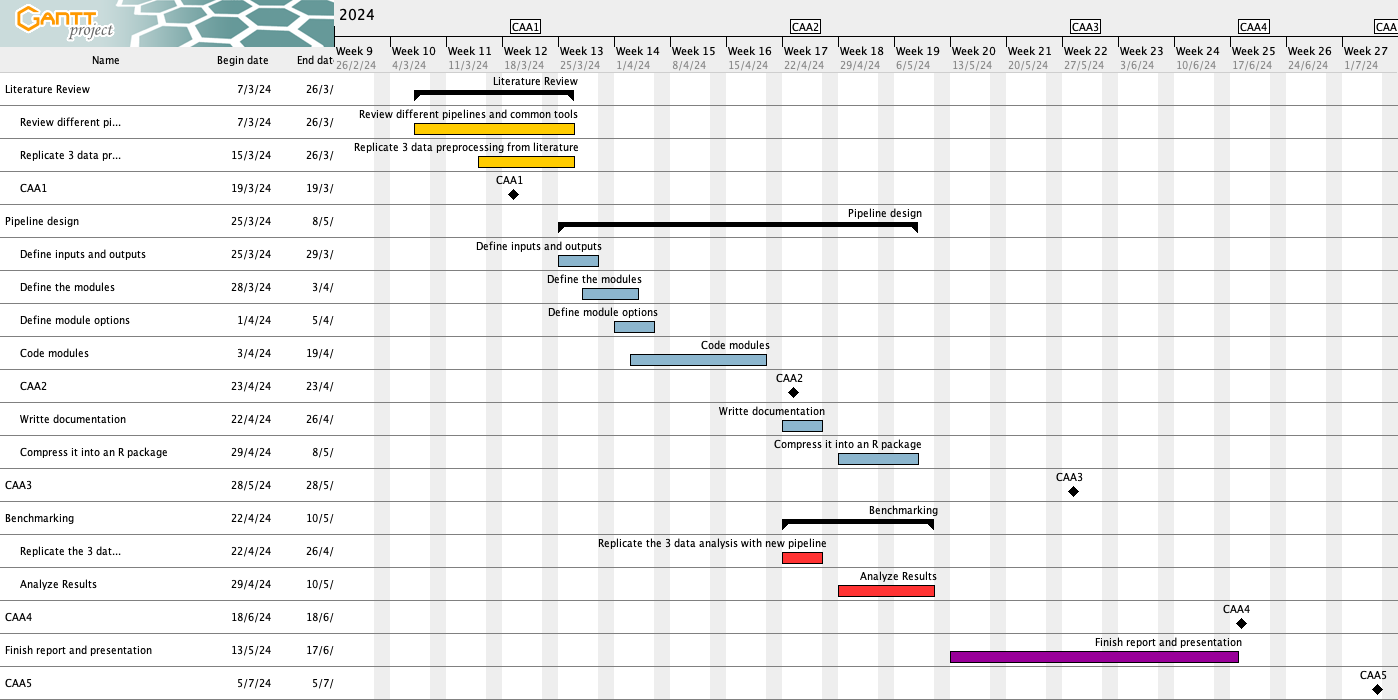
\includegraphics[width=\textwidth]{Images/gantt.png}
    \caption{Gantt chart showing the project timeline and milestones.}
    \label{fig:gantt}
\end{figure}

% \definecolor{gblue}{RGB}{66,133,244}
% \definecolor{gred}{RGB}{234,67,53}
% \definecolor{gyellow}{RGB}{251,188,4}
% \definecolor{ggreen}{RGB}{52,168,83}
% \definecolor{ggrey}{RGB}{154,160,166}
% \definecolor{gblack}{RGB}{32,33,36}
% \definecolor{gorange}{RGB}{227,116,0}

% \begin{landscape}
% \begin{ganttchart}[
%     % expand chart=\textwidth,
%     inline,
%     x unit = 10mm,
%     y unit title=0.5cm,
%     y unit chart=0.5cm,
%     time slot format=isodate-yearmonth,
%     time slot unit=day,
%     % calendar week text={W\currentweek},
%     title/.append style={shape=rectangle, fill=ggrey},
%     title height=1,
%     bar/.append style={fill=gyellow},
%     bar height=.6,
%     bar label font=\normalsize\color{gblack},
%     group top shift=.6,
%     group height=.3,
%     group peaks height=.2,
%     bar incomplete/.append style={fill=ggreen}
% ]{2024-03-05}{2024-07-15}
% \gantttitlecalendar{year, month, day} \\
% \ganttgroup{Literature Review}{2024-03-07}{2024-03-26} \\
%     \ganttbar{Review different pipelines and common tools}{2024-03-07}{2024-03-26}  \\
%     \ganttbar{Replicate 3 data preprocessing from literature}{2024-03-15}   {2024-03-26} \\
%     \ganttmilestone{CAA1}{2024-03-19}{2024-03-19} \\
% \ganttset{bar/.append style={fill=gblue}}
% \ganttgroup{Pipeline design}{2024-03-25}{2024-05-15} \\
%     \ganttbar{Define inputs and outputs}{2024-03-25}{2024-03-29} \\
%     \ganttbar{Define the modules}{2024-03-28}{2024-04-03} \\
%     \ganttbar{Define module options}{2024-04-01}{2024-04-05} \\
%     \ganttbar{Code modules}{2024-04-03}{2024-04-26} \\
%     \ganttbar{Code report}{2024-04-29}{2024-05-06} \\
%     \ganttmilestone{CAA2}{2024-04-23}{2024-04-23} \\
%     \ganttbar{Write documentation}{2024-05-06}{2024-05-15} \\
%     \ganttmilestone{CAA3}{2024-05-28}{2024-05-28} \\

% \ganttset{bar/.append style={fill=gred}}
% \ganttgroup{Benchmarking}{2024-05-13}{2024-05-20} \\
%     \ganttbar{Replicate the 3 data analysis with new pipeline}{2024-05-13}  {2024-05-14} \\
%     \ganttbar{Analyze Results}{2024-05-15}{2024-05-20} \\
%     \ganttmilestone{CAA4}{2024-06-18}{2024-06-18} \\
%     \ganttbar{Finish report and presentation}{2024-05-20}{2024-06-17} \\
%     \ganttmilestone{CAA5}{2024-07-05}{2024-07-05} \\
% \end{ganttchart}
% \end{landscape}
% \restoregeometry

\subsection{Tasks}
\subsubsection{Main Tasks and prioritization}


\subsubsection{Extra tasks}


\section{Risk analysis}

\begin{table}[!h]
    \centering
    \begin{tabular}{|c|c|c|p{6cm}|}
    \hline
    \rowcolor[HTML]{999999} 
    {\color[HTML]{FFFFFF} \textbf{Risk}} &
      {\color[HTML]{FFFFFF} \textbf{Severity}} &
      {\color[HTML]{FFFFFF} \textbf{Likelihood}} &
      \multicolumn{1}{c|}{\cellcolor[HTML]{999999}{\color[HTML]{FFFFFF} \textbf{Mitigation}}} \\ \hline
    \textbf{Resource constraints} &
      \cellcolor[HTML]{FFE599}Moderate &
      \cellcolor[HTML]{FFE599}Moderate &
      Develop a clear project timeline, incorporating milestones and allocating adequate time for each phase. Ensure contingency measures are in place to address unforeseen challenges or changes. \\ \hline
    \textbf{Technical challenges} &
      \cellcolor[HTML]{FFE599}Moderate &
      \cellcolor[HTML]{EA9999}High &
      Perform proper exploration of packages and software and seek guidance and mentorship from professors or experts in relevant fields. \\ \hline
    \textbf{User adoption and awareness} &
      \cellcolor[HTML]{EA9999}High &
      \cellcolor[HTML]{FFE599}Moderate &
      Be sure to incorporate appropriate cautions regarding the correct application of the chosen modules and data. \\ \hline
    \textbf{Pipeline branching} &
      \cellcolor[HTML]{B6D7A8}Low &
      \cellcolor[HTML]{FFE599}Moderate &
      Adopt new methods to interactively select the branching \\ \hline
    \end{tabular}
    \caption{Risk analysis. This table presents various risks associated with the project, along with
    their severity, likelihood, and potential mitigation measures.}
    \label{tab:risk-analysis}
\end{table}



\section{Final products} \todo{Expand on every item}
\begin{itemize}
    \item A pipeline for targeted metabolomic data preprocessing.
    \item A package for the modular implementation of that pipeline in R.
    \item A detailed documentation of the pipeline.
    \item A Shiny app for the accessibility of the pipeline.
    \item A public repository with the code and documentation.
\end{itemize}

\section{Chapters structure} \todo{Dejar para el final}
Breve explicación de los contenidos de cada capítulo y su relación con el proyecto global.



\chapter{Materials and methods}
\todo[inline]{Los aspectos más relevante del diseño y desarrollo del trabajo.}
\todo[inline]{La metodología elegida para hacer este desarrollo, describiendo las alternativas posibles, las decisiones tomadas, y los criterios utilizados para tomar estas decisiones.}
\todo[inline]{Los productos obtenidos}

\section{Datasets} \todo{Data sources and description}
The datasets employed for the purpose of this study were obtained from public repositories.
The datasets were selected based on the following criteria:
\begin{itemize}
    \item Aim of the dataset
    \item Availability of raw data
    \item Targeted metabolomics data
    \item Diverse biological samples
\end{itemize}

The datasets selected were 3:
\begin{itemize}
    \item MTBLS79 \cite{kirwanDirectInfusionMass2014}: This dataset represents a systematic evaluation of the reproducibility of a multi-batch direct-infusion mass spectrometry (DIMS)-based metabolomics study of cardiac tissue extracts. It comprises twenty biological samples (cow vs. sheep) that were analysed repeatedly, in 8 batches across 7 days, together with a concurrent set of quality control (QC) samples. Data are presented from each step of the data processing workflow and are available through MetaboLights.
    \item ST000284 \cite{zhuColorectalCancerDetection2014}
    \item Dataset 3

\end{itemize}
\section{Packages} \todo{Also a brief description of the most relevant ones}
The pipeline was developed using the R programming language \cite{R} and the packages described in \ref{tab:packages}.

\begin{table}[!h]
    \centering
    \begin{tabular}{@{}
    >{\columncolor[HTML]{FFFFFF}}l 
    >{\columncolor[HTML]{FFFFFF}}l 
    >{\columncolor[HTML]{FFFFFF}}c @{}}
    \toprule
    \multicolumn{1}{c}{\cellcolor[HTML]{FFFFFF}\textbf{Package}} & \multicolumn{1}{c}{\cellcolor[HTML]{FFFFFF}\textbf{Version}} & \textbf{Ref}                   \\ \midrule
    {\color[HTML]{000000} arrow}          & {\color[HTML]{000000} \textit{15.0.1}}  & \cite{R-arrow} \\
    {\color[HTML]{000000} base}           & {\color[HTML]{000000} \textit{4.3.3}}   & \cite{R}  \\
    {\color[HTML]{000000} BiocStyle}      & {\color[HTML]{000000} \textit{2.30.0}}  & \cite{R-BiocStyle}  \\
    {\color[HTML]{000000} caret}          & {\color[HTML]{000000} \textit{6.0.94}}  & \cite{R-caret}  \\
    {\color[HTML]{000000} cowplot}        & {\color[HTML]{000000} \textit{1.1.3}}   & \cite{R-cowplot}  \\
    {\color[HTML]{000000} crew}           & {\color[HTML]{000000} \textit{0.9.2}}   & \cite{R-crew}  \\
    {\color[HTML]{000000} datasets}       & {\color[HTML]{000000} \textit{4.3.3}}   & \cite{R}  \\
    {\color[HTML]{000000} dplyr}          & {\color[HTML]{000000} \textit{1.1.4}}   & \cite{R-dplyr}  \\
    {\color[HTML]{000000} DT}             & {\color[HTML]{000000} \textit{0.33}}    & \cite{R-DT}  \\
    {\color[HTML]{000000} fst}            & {\color[HTML]{000000} \textit{0.9.8}}   & \cite{R-fst}  \\
    {\color[HTML]{000000} ggforce}        & {\color[HTML]{000000} \textit{0.4.2}}   & \cite{R-ggforce}  \\
    {\color[HTML]{000000} graphics}       & {\color[HTML]{000000} \textit{4.3.3}}   & \cite{R-graph}  \\
    {\color[HTML]{000000} grDevices}      & {\color[HTML]{000000} \textit{4.3.3}}   & \cite{R}  \\
    {\color[HTML]{000000} HotellingEllipse}                      & {\color[HTML]{000000} \textit{1.1.0}}                        & \cite{R-HotellingEllipse} \\
    {\color[HTML]{000000} impute}         & {\color[HTML]{000000} \textit{1.76.0}}  & \cite{R-impute}  \\
    {\color[HTML]{000000} imputeLCMD}     & {\color[HTML]{000000} \textit{2.1}}     & \cite{R-imputeLCMD}  \\
    {\color[HTML]{000000} knitr}          & {\color[HTML]{000000} \textit{1.46}}    & \cite{R-knitr}  \\
    {\color[HTML]{000000} MetaboAnalystR} & {\color[HTML]{000000} \textit{4.0.0}}   & \cite{R-MetaboAnalystR}  \\
    {\color[HTML]{000000} methods}        & {\color[HTML]{000000} \textit{4.3.3}}   & \cite{R}  \\
    {\color[HTML]{000000} missForest}     & {\color[HTML]{000000} \textit{1.5}}     & \cite{R-missForest}  \\
    {\color[HTML]{000000} pcaMethods}     & {\color[HTML]{000000} \textit{1.94.0}}  & \cite{R-pcaMethods}  \\
    {\color[HTML]{000000} pmp}            & {\color[HTML]{000000} \textit{1.14.1}}  & \cite{R-pmp}  \\
    {\color[HTML]{000000} purrr}          & {\color[HTML]{000000} \textit{1.0.2}}   & \cite{R-purrr}  \\
    {\color[HTML]{000000} renv}           & {\color[HTML]{000000} \textit{1.0.5}}   & \cite{R-renv}  \\
    {\color[HTML]{000000} reshape2}       & {\color[HTML]{000000} \textit{1.4.4}}   & \cite{R-reshape2}  \\
    {\color[HTML]{000000} rmarkdown}      & {\color[HTML]{000000} \textit{2.26}}    & \cite{R-rmarkdown}  \\
    {\color[HTML]{000000} shiny}          & {\color[HTML]{000000} \textit{1.8.1.1}} & \cite{R-shiny}  \\
    {\color[HTML]{000000} shinyFiles}     & {\color[HTML]{000000} \textit{0.9.3}}   & \cite{R-shinyFiles}  \\
    {\color[HTML]{000000} stats}          & {\color[HTML]{000000} \textit{4.3.3}}   & \cite{R}  \\
    {\color[HTML]{000000} structToolbox}  & {\color[HTML]{000000} \textit{1.14.0}}  & \cite{R-structToolbox}  \\
    {\color[HTML]{000000} SummarizedExperiment}                  & {\color[HTML]{000000} \textit{1.32.0}}                       & \cite{R-SummarizedExperiment} \\
    {\color[HTML]{000000} tarchetypes}    & {\color[HTML]{000000} \textit{0.9.0}}   & \cite{R-tarchetypes}  \\
    {\color[HTML]{000000} targets}        & {\color[HTML]{000000} \textit{1.6.0}}   & \cite{R-targets}  \\
    {\color[HTML]{000000} tidyverse}      & {\color[HTML]{000000} \textit{2.0.0}}   & \cite{R-tidyverse}  \\
    {\color[HTML]{000000} tinytex}        & {\color[HTML]{000000} \textit{0.51}}    & \cite{R-tinytex}  \\
    {\color[HTML]{000000} tools}          & {\color[HTML]{000000} \textit{4.3.3}}   & \cite{R}  \\
    {\color[HTML]{000000} usethis}        & {\color[HTML]{000000} \textit{2.2.3}}   & \cite{R-usethis}  \\
    {\color[HTML]{000000} utils}          & {\color[HTML]{000000} \textit{4.3.3}}   & \cite{R}  \\
    {\color[HTML]{000000} VIM}            & {\color[HTML]{000000} \textit{6.2.2}}   & \cite{R-VIM}  \\
    {\color[HTML]{000000} withr}          & {\color[HTML]{000000} \textit{3.0.0}}   & \cite{R-withr}  \\ \bottomrule
    \end{tabular}
    \caption{List of R packages with their versions used to develop \texttt{metaboPipe}}
    \label{tab:packages}
    \end{table}


\todo{add a summary of 1: Number of functions and 2: Number of lines of code}
In this project, we developed an R package named \texttt{metaboPipe} to preprocess metabolomic data efficiently and accessibly. Metabolomic data preprocessing is a crucial step in ensuring the quality and reliability of downstream analyses. The transformations applied during preprocessing are primarily intended to remove unwanted effects unrelated to the study, but these tools can inadvertently delete meaningful biological data if used without caution. The \texttt{metaboPipe} package leverages the \texttt{targets} and \texttt{structToolbox} packages to create a modular and reproducible pipeline for preprocessing. This section details the components and functionality of \texttt{metaboPipe}.

\section{Package Overview}
The \texttt{metaboPipe} package is designed to streamline the preprocessing of metabolomic data by creating a series of user-accessible modules that translate into interconnected steps. These steps can be easily added, modified, and rearranged. The package utilizes the \texttt{targets} package to orchestrate task deployment and dependencies, ensuring that each step is executed in the correct order. The \texttt{structToolbox} package provides the \texttt{DatasetExperiment} object, which serves as the primary data structure throughout the pipeline, along with multiple functions for data transformation.

\section{Functions and Processing Steps}
Although the \texttt{metaboPipe} package comprises over 56 functions, there are six main preprocessing functions that users will primarily engage with, each responsible for a specific data transformation step. These functions are designed to operate sequentially on a \texttt{DatasetExperiment} object, transforming it at each stage to prepare it for subsequent steps.

\subsection{Data Format}
Data must be imported in \texttt{.csv} format, consisting of two types of files:

\subsubsection{Matrix Data}
The matrix data is a table where each row represents a unique sample and each column represents a metabolite. The first row must contain the metabolite names. This table has the concentration data, peak intensity tables or MS/NMR spectral bins

\subsubsection{Sample Metadata}
The sample metadata is a table where each row represents a unique sample and each column represents a variable. The samples must be in the same order as the matrix data. The first row must contain the variable names, and there must be a column named \texttt{sample\_id} specifying a unique identifier for each sample. The number of variables depends on the study and preprocessing needs.

\subsubsection{Feature Metadata}
The feature metadata is an optional table where each row represents a feature and each column information related to the feature such as the chemical formula, retention time, and mass-to-charge ratio. The first row contains the column names and the first column needs to be called \texttt{annotation} containing the feature names. This table is optional as if not provided the pipeline will create a minimum table with only the annotation column using those provided in the matrix data.


\subsection{Data loading}
The data loading function takes the data matrix, sample metadata and optionally a feature metadata files and creates a \texttt{DatasetExperiment} object providing a structured representation of the metabolomic dataset. Loading the data is the first step in the preprocessing pipeline, enabling the subsequent transformations to be applied to the data.

\subsection{Filtering}
Filtering is usually the first step in the pipeline. It removes irrelevant or low-quality features from the dataset based on user-defined criteria. This step is essential to reduce noise and enhance the accuracy of downstream analyses.
The module generates target nodes that apply the filtering criteria to the
\texttt{DatasetExperiment} object, producing a refined dataset. Those criteria are the minimum percentage of samples and metabolites with non-zero values and the removing of outliers based on the Hotelling's T2 distribution ellipse.



\subsection{Imputation} 
Following filtering, the imputation function addresses missing values in the dataset. Missing data can significantly affect the results of metabolomic analyses; hence, accurate imputation is critical. The imputation function offers various methods for estimating missing values, such as mean substitution, k-nearest neighbors, and multiple imputation, and updates the \texttt{DatasetExperiment} object accordingly. 

\subsection{Batch Correction} 
Batch effects are common in metabolomic studies and can confound results if not properly corrected. The batch correction function in \texttt{metaboPipe} identifies and adjusts for batch effects, ensuring that the data is comparable across different experimental batches. This step generates target nodes that modify the \texttt{DatasetExperiment} object to remove batch-related variability. 

\subsection{Normalization} 
Normalization is performed to account for differences in sample concentration and ensure that the metabolite intensities are comparable across samples. The normalization function offers several methods, including total area normalization, probabilistic quotient normalization, and variance stabilization. The normalized \texttt{DatasetExperiment} object is then passed to the next processing step.


\subsection{Scaling} 
Scaling is used to adjust the range and distribution of metabolite intensities. The scaling function in \texttt{metaboPipe} provides options such as standard scaling (z-score), min-max scaling, and Pareto scaling. This step standardizes the data, facilitating meaningful comparisons between metabolites. The scaled \texttt{DatasetExperiment} object is prepared for the final transformation step. 

\subsection{Transformation} 
The transformation function applies mathematical transformations to stabilize the variance and make the data more normally distributed. Common transformations include logarithmic, square root, and Box-Cox transformations. The transformed \texttt{DatasetExperiment} object is the final output of the preprocessing pipeline, ready for downstream analysis. 

\section{Implementation Details}
Each preprocessing step in \texttt{metaboPipe} is implemented as a function that creates target nodes using the \texttt{targets} package. These nodes encapsulate the necessary operations and dependencies, ensuring that the pipeline is both modular and reproducible. 

The \texttt{DatasetExperiment} object from the \texttt{structToolbox} package is used throughout the pipeline, providing a consistent and flexible data structure for all preprocessing steps.


\section{Conclusion} 
The \texttt{metaboPipe} package offers a comprehensive and modular approach to preprocessing metabolomic data. By integrating the \texttt{targets} and \texttt{structToolbox} packages, \texttt{metaboPipe} ensures that each preprocessing step is executed efficiently and reproducibly. This pipeline enhances the quality of metabolomic data, facilitating robust and reliable downstream analyses. Future work may involve extending the pipeline to include additional preprocessing steps or integrating advanced machine learning techniques for enhanced data processing.




\section{Documentation}


\section{Shiny app}
 


\chapter{Results}

Detallad en este apartado los resultados obtenidos utilizando la metodología descrita en el apartado anterior.

Las figuras tienen que estar explicadas y citadas en el texto, como la \ref{fig:my_label}, en la cual se muestra el error en función de la distancia, en unidades arbitrarias. En todas las gráficas tiene que haber el título de los ejes.

\begin{figure}[!htbp]
    \centering
    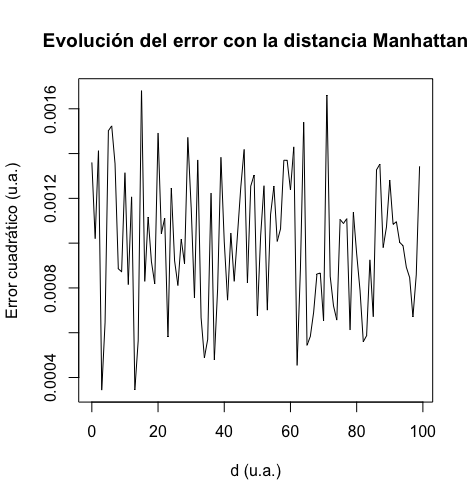
\includegraphics[width=7truecm]{Template/Rplotmanh.png}
    \caption{Error en función de la distancia en unidades arbitrarias.}
    \label{fig:my_label}
\end{figure}

%\chapter{Discusión}
%Discusión de los resultados en el contexto del proyecto. Es en este apartado donde cobran sentido y en el cual se responden las preguntas de investigación y se muestra como los resultados dan respuesta a los problemas planteados.

%Esta parte puede ser que no aplique según el tipo de trabajo.

%\chapter{Valoración económica}
%En caso de que corresponda, se incluirá un apartado de ``Valoración económica del trabajo". Este apartado indicará los gastos asociados al desarrollo y mantenimiento del trabajo, así como los beneficios económicos obtenidos. Hay que hacer un análisis final sobre la viabilidad del producto.

\chapter{Conclusion and future vision}

%\section{Conclusiones}
Este capítulo tiene que incluir:
\begin{itemize}
\item Una descripción de las conclusiones del trabajo:
\begin{itemize}
    \item Una vez se han obtenido los resultados, ¿qué conclusiones se extraen?
    \item ¿Estos resultados son los esperados? ¿O han sido sorprendentes? ¿Por qué? 
\end{itemize}
\item Una reflexión crítica sobre el logro de los objetivos planteados inicialmente:
\begin{itemize}
    \item ¿Hemos logrado todos los objetivos? Si la respuesta es negativa, ¿por qué motivo?
\end{itemize}
\item Un análisis crítico del seguimiento de la planificación y metodología a lo largo del producto:
\begin{itemize}
    \item ¿Se ha seguido la planificación?
    \item ¿La metodología prevista ha sido suficientemente adecuada?
    \item ¿Ha habido que introducir cambios para garantizar el éxito del trabajo? ¿Por qué? 
\end{itemize}
\item De los impactos previstos en \ref{s:etic}, ético-sociales, de sostenibilidad y de diversidad, evaluar/mencionar si se han mitigado (si eran negativos) o si se han conseguido (si eran positivos). 
\item Si han aparecido impactos no previstos a \ref{s:etic}, evaluar/mencionar cómo se han mitigado (si eran negativos) o que han aportado (si eran positivos).
\item Las líneas de trabajo futuro que no se han podido explorar en este trabajo y han quedado pendientes.
\item Glossary test:  \gls{latex}


%\item Una descripción de las conclusiones del trabajo: Qué lecciones se han aprendido del trabajo?
%\item Una reflexión crítica sobre el logro de los objetivos planteados inicialmente: Hemos conseguido todos los objetivos? Si la respuesta es negativa, por qué motivo?
%\item De los impactos previstos a la sección \ref{s:etic}, una evaluación, o al menos, mención, sobre si se han mitigado (si eran negativos) o si se han conseguido (si eran positivos). 
\end{itemize}

%\section{Líneas de futuro}
%Las líneas de trabajo futuro que no se han podido explorar en este trabajo y han quedado pendientes.

%\section{Seguimiento de la planificación}
%Un análisis crítico del seguimiento de la planificación y metodología a lo largo del trabajo: 
%\begin{itemize}
%    \item  Se ha seguido la planificación? 
%    \item La metodología prevista ha sido la adecuada? 
%    \item Ha habido que introducir cambios para garantizar el éxito del trabajo? ¿Por qué? 
%\end{itemize}

\setglossarystyle{list}
\printglossary[title=Glossary, toctitle=Glossary]
\printglossary[type=\acronymtype, title=Acronyms, toctitle=Acronyms]



\printbibliography[heading=bibintoc]


\newpage
\appendix
Listado de apartados que son demasiado extensos para incluir dentro de la memoria y tienen un carácter autocontenido (por ejemplo, manuales de usuario, manuales de instalación, etc.)
 
Dependiendo del tipo de trabajo, es posible que no haya que añadir algún anexo.

\end{document}
